\newpage
\section{RESULT AND DISCUSSION}
Here, We will discuss how different models performed when compared to each other. We compare them using PSNR and SSIM in different test sets. Since, these metrics don't tell the complete picture we have provided the comparison images from different models here.
\subsection{Evaluation Metrics}
We calculated PSNR and SSIM for all the test datasets Set5, Set14 and BSDS100 after the training was completed with each model.
\begin{table}[h]
    \centering
    \begin{tabular}{|c|c|c|c|c|c|c|}
    \hline
    &PSNR & SISM & PSNR & SISM & PSNR & SISM \\
    \hline
    SRCNN(3x)&31.02 & 0.9 & 27.668 & 0.812 & 26.939 & 0.781 \\
    \hline
    SRCNN(4x)&28.751 & 0.844 & 25.72 & 0.734 & 25.44 & 0.696 \\
    \hline
    ResNet&29.83 & 0.887 & 28.275 & 0.795 & 27.203 & 0.751 \\
    \hline
    SRGAN &26.132 & 0.821 &25.684 & 0.716 & 24.969 & 0.665 \\
    \hline
    & \multicolumn{2}{|c|}{Set5}& \multicolumn{2}{|c|}{Set14} & \multicolumn{2}{|c|}{BSD100} \\
    \hline
    \end{tabular}
    \caption{Evaluation Metrics in Test Datasets}
\end{table}
\clearpage
% Table
During Training We calculated PSNR and SSIM for Set5 datasets at every epoch for both SRResNet and SRGAN.
\begin{figure}[h]
    \centering
    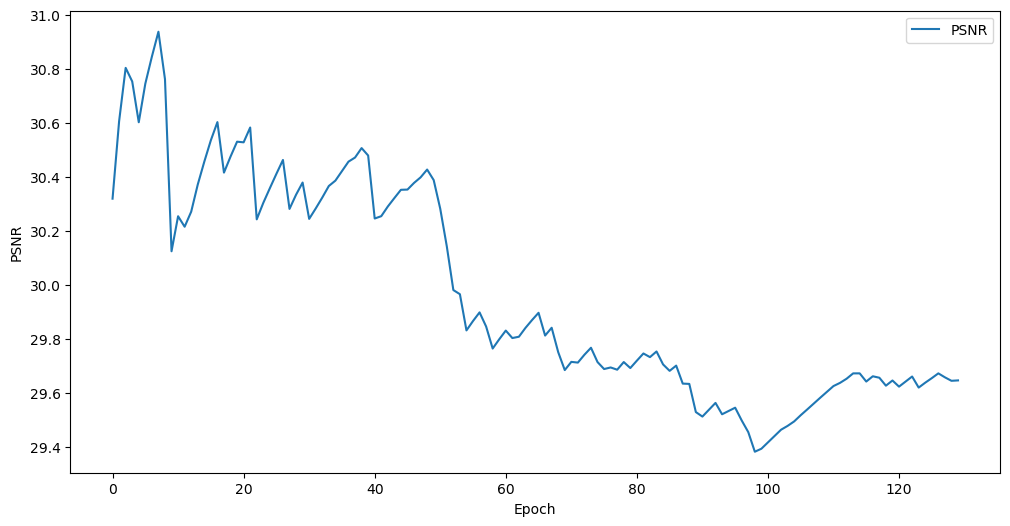
\includegraphics[width=5.5in]{./figures/srresnet_psnr.png}
    % \caption{SRResNet PSNR Plot}
    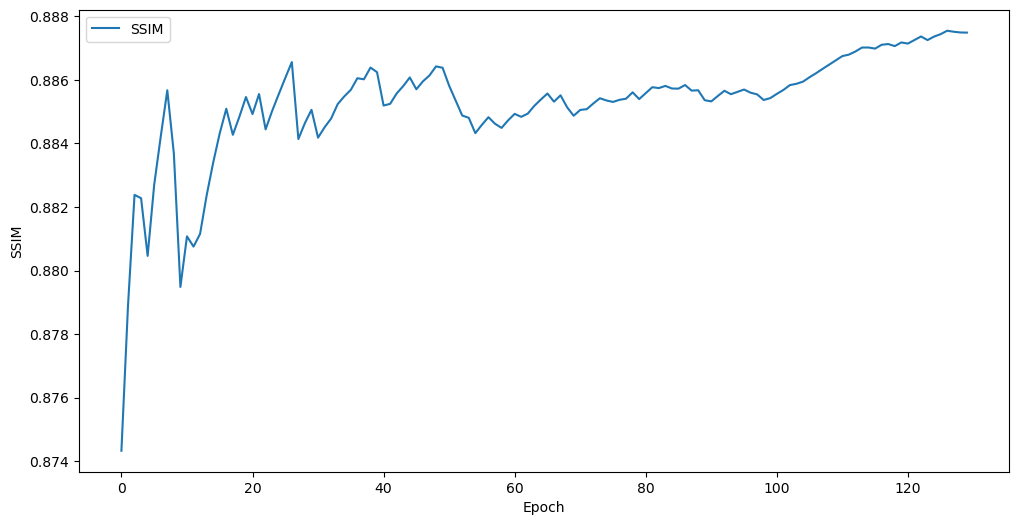
\includegraphics[width=5.5in]{./figures/srresnnet_ssim.png}
    \caption{SRResNet PSNR and SSIM Plot for Set5}
\end{figure}  
\begin{figure}[h]
    \centering
    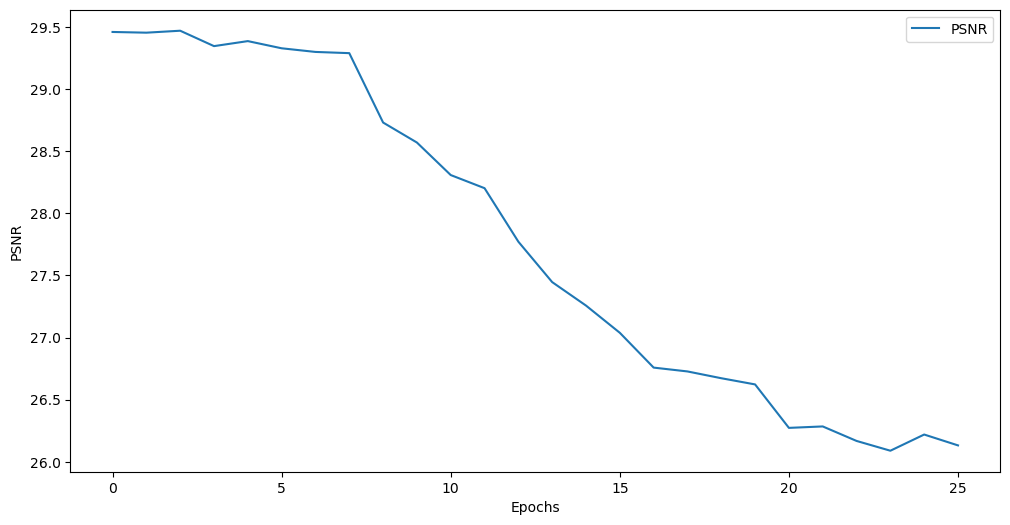
\includegraphics[width=5.5in]{./figures/srgan_psnr.png}
    % \caption{SRResNet PSNR Plot}
    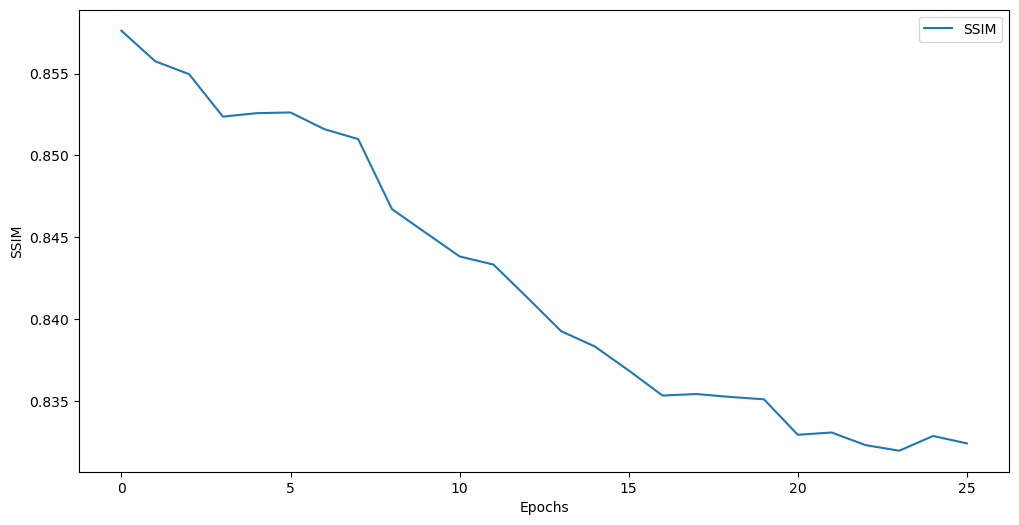
\includegraphics[width=5.5in]{./figures/srgan_ssim.png}
    \caption{SRGAN PSNR and SSIM Plot for Set5}
\end{figure}  
\begin{figure}[h]
    \centering
    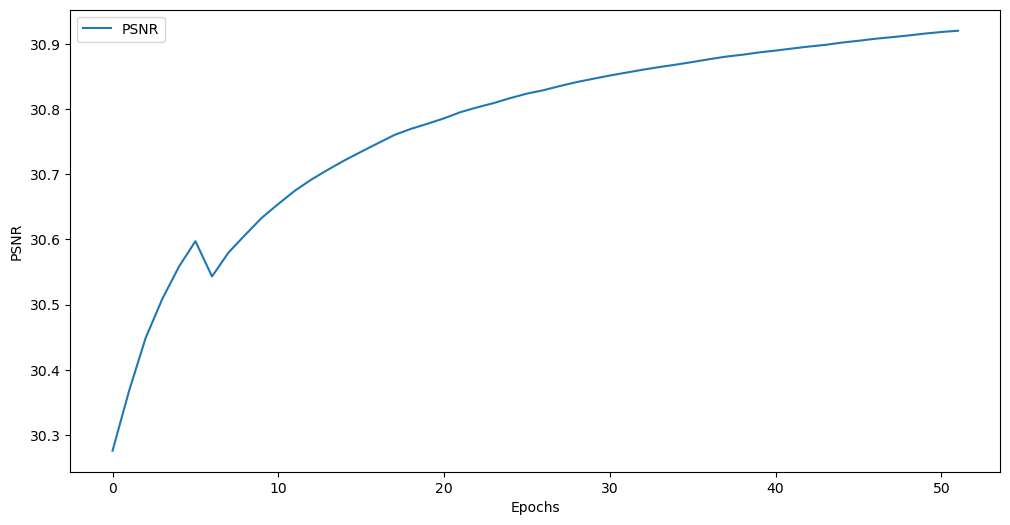
\includegraphics[width=5.5in]{./figures/SRCNN_PSNR.png}
    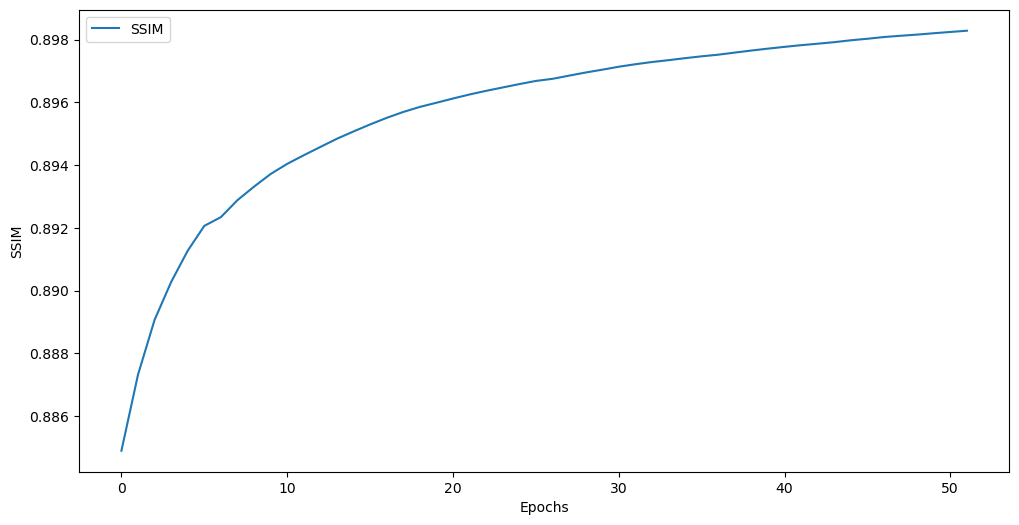
\includegraphics[width=5.5in]{./figures/SRCNN_SSIM.png}
    \caption{SRCNN PSNR and SSIM Plot for Set5}
\end{figure} 
    These metrics don't actually match with human perception but even if PSNR and SSIM is decreasing they are becoming more stable and we see model get better after each epoch.
\clearpage
\newpage
\subsection{Image Comparsions}
    These are the few results from comparing Bicubic, SRResNet and SRGAN super resolved images with the original HR images.
    \begin{figure}
        \centering
        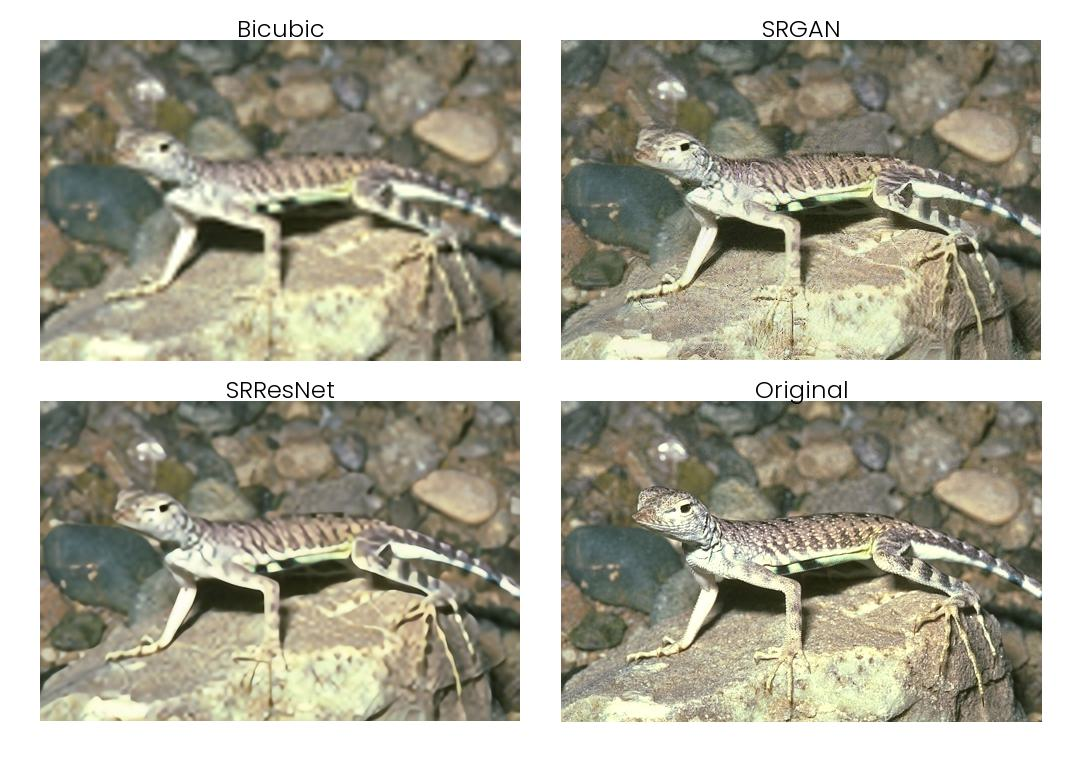
\includegraphics[width=5.5in]{./figures/examples/lizard.jpg}
        \caption{Image of super resolved lizard with SRResNet, SRGAN and HR image}
    \end{figure}
    \begin{figure}
        \centering
        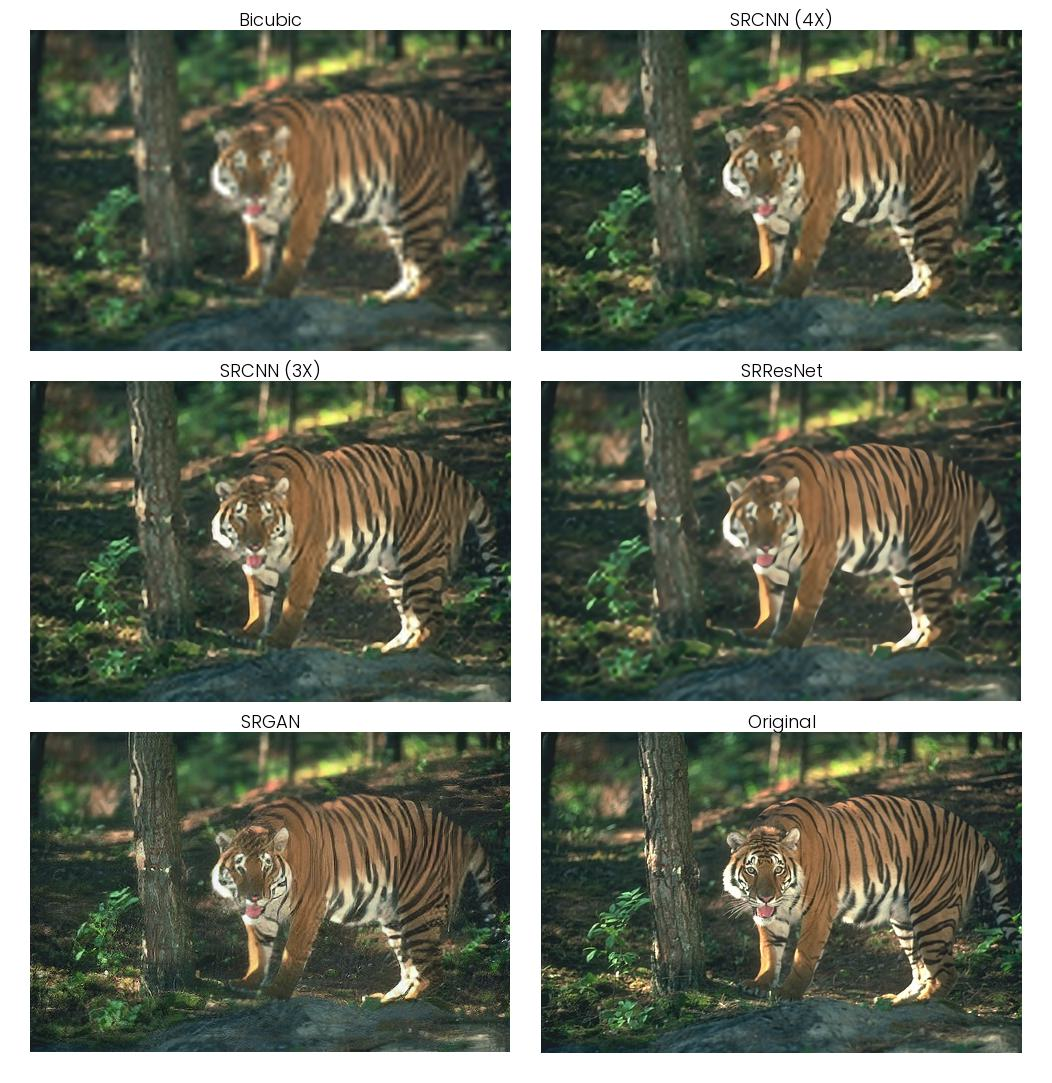
\includegraphics[width=5.5in]{./figures/examples/tiger.jpg}
        \caption{Images of super resolved tiger with SRResNet, SRGAN and HR image}
    \end{figure}
    \begin{figure}
        \centering
        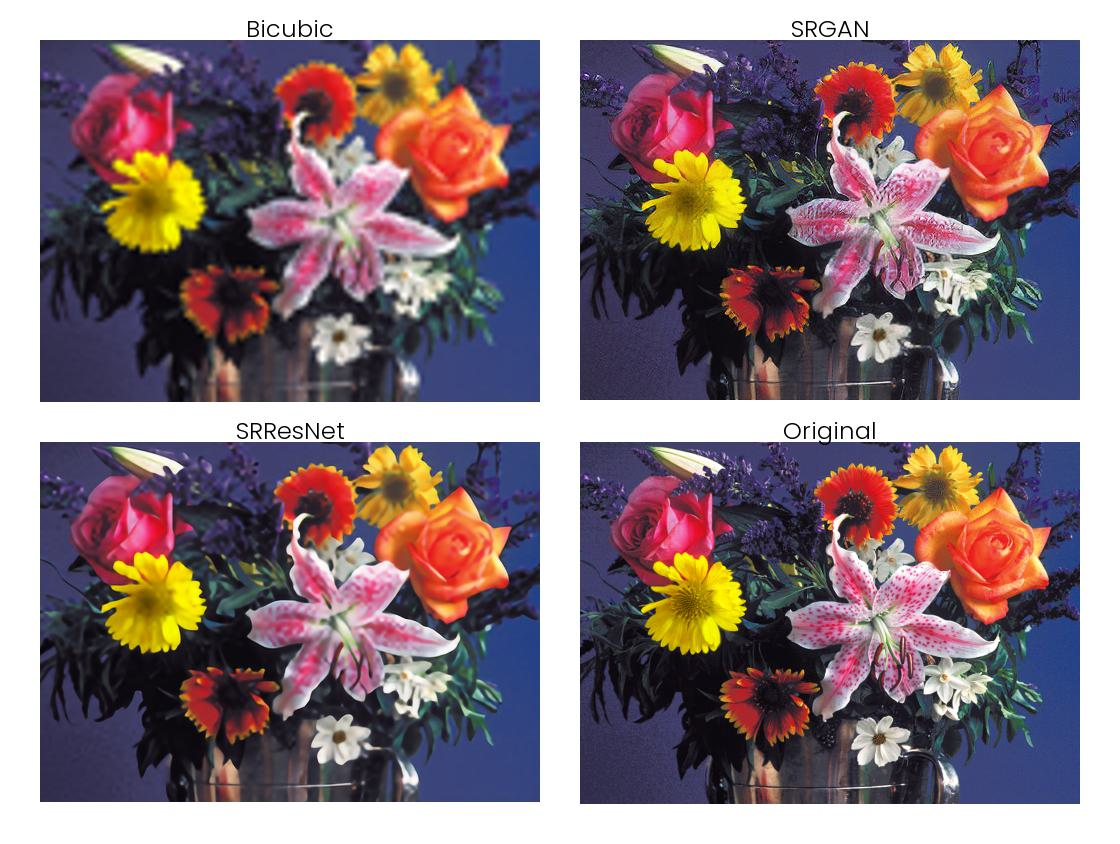
\includegraphics[width=5.5in]{./figures/examples/flowers.jpg}
        \caption{Images of super resolved flowers  with SRResNet, SRGAN and HR image}
    \end{figure}       
  
\clearpage
\newpage
\subsection{Recommendation}
From our observations, when one needs to do 2x upscaling there is no need for a NN model, We can simply use Bicubic Interpolation if there is enough details present in low resolution image. We found NN models more important and useful when upscaling 3x and 4x. SRCNN models are simple convolutional neural networks, They can't perform in the league of SRResNet and SRGAN when 4x upscaling. But SRCNN model use very less resources and We recommend use SRCNN for upto 3x upscaling. And for SRResNet and SRGAN they are both resource intensive and SRGAN takes very long to train even more than SRResNet. They perform well in 4x upscaling also specially SRGAN. We recommend the use of SRGAN for scaling above 3x.
\subsection{Future Enhancements}
We can improve our project by doing following things:
\begin{enumerate}
    \item We only used Y-channel for training SRCNN model, We can use pretrained model in Y-channel and train it in all 3 YCbCr channels for better result.
    \item Data is always a limitation for deep learning models, The models will always perform better if we include more diverse images.
    \item There is a lot of subjectivity in evaluating the images as quantitative metrics can't identify human perception, We can use Mean Opinion Score like metric that can be used to compare different models and their performance.
    \item  We can implment ESRGAN and transformer model like xx for better comparison.
\end{enumerate}
\subsection{Work Schedule:}
\newcolumntype{P}[1]{>{\raggedright\vrule height4ex width 0pt}p{#1}<{\vrule depth 2.5ex width 0pt}}
    \begin{tabular}{|P{6cm}*{10}{|c}|}
    \hline
    \centering \raisebox{-2ex}[0pt][0pt]{Action plan} & \multicolumn{7}{c|}{2023} & \multicolumn{3}{c|}{2024} \\
    \cline{2-11}
    \multicolumn{1}{|c|}{\vphantom{$\Big|$}} &
    \scriptsize Jun & \scriptsize Jul & \scriptsize Aug & \scriptsize Sep &
    \scriptsize Oct & \scriptsize Nov & \scriptsize Dec & \scriptsize Jan &
    \scriptsize Feb & \scriptsize Mar \\
    \hline
    Research &
    {\cellcolor{gray}} &{\cellcolor{gray}}&{\cellcolor{gray}}&{\cellcolor{gray}}&{\cellcolor{gray}}&&&&& \\
    \hline
    Data Acquisition &
    && {\cellcolor{gray}} &{\cellcolor{gray}} &{\cellcolor{gray}} &&&&& \\
    \hline
    Model Development and Evaluation &
    &&&&{\cellcolor{gray}} &{\cellcolor{gray}}&{\cellcolor{gray}}&&& \\
    \hline
    Model Deployment &
    &&&&&&{\cellcolor{gray}}&{\cellcolor{gray}}&{\cellcolor{gray}} & \\
    \hline
    Prepare the report and presentation &
    &&&&&&{\cellcolor{gray}}&{\cellcolor{gray}}&{\cellcolor{gray}}&{\cellcolor{gray}} \\
    \hline
    \end{tabular}